%Randy Schur

%format based on:
%% bare_jrnl.tex
%% V1.4b
%% 2015/08/26
%% by Michael Shell
%% see http://www.michaelshell.org/
%% for current contact information.
%%
%% This is a skeleton file demonstrating the use of IEEEtran.cls
%% (requires IEEEtran.cls version 1.8b or later) with an IEEE
%% journal paper.
%%
%% Support sites:
%% http://www.michaelshell.org/tex/ieeetran/
%% http://www.ctan.org/pkg/ieeetran
%% and
%% http://www.ieee.org/

%%*************************************************************************
%% Legal Notice:
%% This code is offered as-is without any warranty either expressed or
%% implied; without even the implied warranty of MERCHANTABILITY or
%% FITNESS FOR A PARTICULAR PURPOSE! 
%% User assumes all risk.
%% In no event shall the IEEE or any contributor to this code be liable for
%% any damages or losses, including, but not limited to, incidental,
%% consequential, or any other damages, resulting from the use or misuse
%% of any information contained here.
%%
%% All comments are the opinions of their respective authors and are not
%% necessarily endorsed by the IEEE.
%%
%% This work is distributed under the LaTeX Project Public License (LPPL)
%% ( http://www.latex-project.org/ ) version 1.3, and may be freely used,
%% distributed and modified. A copy of the LPPL, version 1.3, is included
%% in the base LaTeX documentation of all distributions of LaTeX released
%% 2003/12/01 or later.
%% Retain all contribution notices and credits.
%% ** Modified files should be clearly indicated as such, including  **
%% ** renaming them and changing author support contact information. **
%%*************************************************************************


% *** Authors should verify (and, if needed, correct) their LaTeX system  ***
% *** with the testflow diagnostic prior to trusting their LaTeX platform ***
% *** with production work. The IEEE's font choices and paper sizes can   ***
% *** trigger bugs that do not appear when using other class files.       ***                          ***
% The testflow support page is at:
% http://www.michaelshell.org/tex/testflow/



\documentclass[journal]{IEEEtran}
% *** CITATION PACKAGES ***
%
\usepackage{cite}
%\renewcommand*{\citen}[1]{%
%  \begingroup
%    \romannumeral-`\x % remove space at the beginning of \setcitestyle
%    \setcitestyle{numbers}%
%    \cite{#1}%
%  \endgroup   
%}
% cite.sty was written by Donald Arseneau
% V1.6 and later of IEEEtran pre-defines the format of the cite.sty package
% \cite{} output to follow that of the IEEE. Loading the cite package will
% result in citation numbers being automatically sorted and properly
% "compressed/ranged". e.g., [1], [9], [2], [7], [5], [6] without using
% cite.sty will become [1], [2], [5]--[7], [9] using cite.sty. cite.sty's
% \cite will automatically add leading space, if needed. Use cite.sty's
% noadjust option (cite.sty V3.8 and later) if you want to turn this off
% such as if a citation ever needs to be enclosed in parenthesis.
% cite.sty is already installed on most LaTeX systems. Be sure and use
% version 5.0 (2009-03-20) and later if using hyperref.sty.
% The latest version can be obtained at:
% http://www.ctan.org/pkg/cite
% The documentation is contained in the cite.sty file itself.

\makeatletter
\renewcommand{\@IEEEsectpunct}{\ }% Modified from {:\ \,}

%\makeatother




% *** GRAPHICS RELATED PACKAGES ***

\usepackage[pdftex]{graphicx}
\usepackage{amsmath}
\interdisplaylinepenalty=2500


\usepackage{algorithmic}
\usepackage{array}
\usepackage{tikz}
\usetikzlibrary{positioning}

\renewcommand{\algorithmiccomment}[1]{// #1}
\newcounter{row}
\newcounter{col}

% *** SUBFIGURE PACKAGES ***
%\ifCLASSOPTIONcompsoc
%  \usepackage[caption=false,font=normalsize,labelfont=sf,textfont=sf]{subfig}
%\else
%  \usepackage[caption=false,font=footnotesize]{subfig}
%\fi
% subfig.sty, written by Steven Douglas Cochran, is the modern replacement
% for subfigure.sty, the latter of which is no longer maintained and is
% incompatible with some LaTeX packages including fixltx2e. However,
% subfig.sty requires and automatically loads Axel Sommerfeldt's caption.sty
% which will override IEEEtran.cls' handling of captions and this will result
% in non-IEEE style figure/table captions. To prevent this problem, be sure
% and invoke subfig.sty's "caption=false" package option (available since
% subfig.sty version 1.3, 2005/06/28) as this is will preserve IEEEtran.cls
% handling of captions.
% Note that the Computer Society format requires a larger sans serif font
% than the serif footnote size font used in traditional IEEE formatting
% and thus the need to invoke different subfig.sty package options depending
% on whether compsoc mode has been enabled.
%
% The latest version and documentation of subfig.sty can be obtained at:
% http://www.ctan.org/pkg/subfig



%\usepackage{stfloats}
% stfloats.sty was written by Sigitas Tolusis. This package gives LaTeX2e
% the ability to do double column floats at the bottom of the page as well
% as the top. (e.g., "\begin{figure*}[!b]" is not normally possible in
% LaTeX2e). It also provides a command:
%\fnbelowfloat
% to enable the placement of footnotes below bottom floats (the standard
% LaTeX2e kernel puts them above bottom floats). This is an invasive package
% which rewrites many portions of the LaTeX2e float routines. It may not work
% with other packages that modify the LaTeX2e float routines. The latest
% version and documentation can be obtained at:
% http://www.ctan.org/pkg/stfloats
% Do not use the stfloats baselinefloat ability as the IEEE does not allow
% \baselineskip to stretch. Authors submitting work to the IEEE should note
% that the IEEE rarely uses double column equations and that authors should try
% to avoid such use. Do not be tempted to use the cuted.sty or midfloat.sty
% packages (also by Sigitas Tolusis) as the IEEE does not format its papers in
% such ways.
% Do not attempt to use stfloats with fixltx2e as they are incompatible.
% Instead, use Morten Hogholm'a dblfloatfix which combines the features
% of both fixltx2e and stfloats:
%
% \usepackage{dblfloatfix}
% The latest version can be found at:
% http://www.ctan.org/pkg/dblfloatfix


% correct bad hyphenation here
\hyphenation{op-tical net-works semi-conduc-tor}

\begin{document}

\title{Dynamic Programming Method for Energy-Aware Path Planning}

% author names and IEEE memberships
% note positions of commas and nonbreaking spaces ( ~ ) LaTeX will not break
% a structure at a ~ so this keeps an author's name from being broken across
% two lines.
% use \thanks{} to gain access to the first footnote area
% a separate \thanks must be used for each paragraph as LaTeX2e's \thanks
% was not built to handle multiple paragraphs
%

\author{Randall~Schur, Conor~Lyman,
        and~Adam~M.~Wickenheiser
%\thanks{M. Shell was with the Department
%of Electrical and Computer Engineering, Georgia Institute of Technology, Atlanta,
%GA, 30332 USA e-mail: (see http://www.michaelshell.org/contact.html).}% <-this % stops a space
%\thanks{J. Doe and J. Doe are with Anonymous University.}% <-this % stops a space
%\thanks{Manuscript received April 19, 2005; revised August 26, 2015.}
}

% The paper headers
%\markboth{Journal of \LaTeX\ Class Files,~Vol.~14, No.~8, August~2015}%
%{Shell \MakeLowercase{\textit{et al.}}: Bare Demo of IEEEtran.cls for IEEE Journals}

\markboth{IEEE Transactions on Robotics Full Paper Submission}%
{Schur \MakeLowercase{\textit{et al.}}: Dynamic Programming Method for Energy-Aware Path Planning}

% make the title area
\maketitle

\begin{abstract}
This paper presents Energy Aware Path Planning (EAPP), a path planning algorithm for mobile robots deployed in extended missions. Battery constraints are often the limiting factor for the range and length of deployment in ground vehicles. In order to extend the lifetime of a mobile robot, solar panels or other energy transducers can be attached to the robot to harvest energy from the environment. The environment may not be well defined; this approach assumes the availability of satellite images which can be segmented into grids, but requires no additional information about obstacles. Our approach defines a novel description of the environment consisting of two costs associated with each grid cell: an energy-based cost of traverse and a collision-based probability of traverse calculated from the model of the robot and the environment. The proposed algorithm takes a dynamic programming approach to finding the least-energy path through the environment without violating a constraint on probability of traverse. Simulations and experiments show more efficient paths for robots in target environments.
\end{abstract}

% Note that keywords are not normally used for peerreview papers.
%\begin{IEEEkeywords}
%IEEE, IEEEtran, journal, \LaTeX, paper, template.
%\end{IEEEkeywords}

% For peerreview papers, this IEEEtran command inserts a page break and
% creates the second title. It will be ignored for other modes.
\IEEEpeerreviewmaketitle



\section{Introduction}
\IEEEPARstart{N}{avigation} algorithms for mobile robots in realistic scenarios present multi-objective optimization problems. 
The goal is to minimize some cost function while maximizing the chances of success. 
In a real-world problem, this means synthesizing incomplete and potentially incorrect information about the environment, while minimizing the cost of executing the final path. 
The cost function may have competing goals; decreasing probability of collision (defined in this study as any obstacle that can damage the robot or stop it from driving), optimizing distance traveled or information gained, minimizing energy usage, or minimizing the time of traverse to a desired region are all potential objectives of the algorithm.
As these are often competing interests, the cost function must weight each objective according to the application, along with the uncertainty associated with each piece of information. 

These competing costs are often difficult to sum into a scalar cost with a single function. The approach presented in this paper, called Energy-Aware Path Planning (EAPP), presents a novel context for characterizing the environment by introducing multiple metrics to describe cost and uncertainty. 
EAPP, considers the case of extended deployment in a partially unknown environment. 
The scenario targeted by this approach is a robot that is deployed on a continuous, extended, and autonomous basis. 
Using robots for applications such as inspection of infrastructure (especially pipelines, bridges, or roads), environmental monitoring and data collection in remote areas, and surveillance \cite{wickenheiser2010design} all require this type of long-term autonomy. 
First and foremost for these applications the robot must continue running and must approach a goal location, and any other goal is secondary. 
This means that two objectives must be considered: minimizing collisions and minimizing energy usage. 
Energy minimization here is important for extended duration missions, as on-board battery storage is often a limiting factor for mobile robot deployment. 
More energy-dense solutions such as fuel cells or radioactive power sources are often impractical due to safety and cost concerns. 
This approach assumes a battery powered vehicle with the addition of energy-harvesting equipment such as a solar panel. 
EAPP segments the map into grid cells and evaluates the competing objectives using both a cost function based on estimated energy usage and a penalty function based on estimated probability of a successful traverse. 
This approach calculates the most efficient path through a cell which does not violate the defined threshold on the likelihood of collision.

Rather than attempting to define a cell by its coverage of obstacles or by the uncertainty in the position of obstacles as in cell decomposition methods \cite{mobile robotics textbook}, probability of traverse ($P_{tr}(x)$) is defined as the estimate of the likelihood that the robot will be able to traverse through the map segment. 
The presence of any obstacle that impedes the robot's motion means that there is some probability the robot will fail to traverse the cell. 
Probability of traverse is a pre-calculated metric related to chance constraints \cite{blackmore2006probabilistic}, although it is not an exact parallel. 
An obstacle density ($\mu(x)$) is also estimated for each map segment, which is used in the calculation of the cost function. 
Separating these metrics allows the explicit calculation of both the cost function (which is additive) and probability of traverse (which is multiplicative) for a path. 

\section{Related Work}

In this paper we focus on go-to-goal behavior for navigation, in particular moving a wheeled robot through an environment from its present location to some target. 
The many approaches to this problem are typically categorized as either probabilistic or deterministic \cite{lavalle2006planning}. 

Probabilistic navigation algorithms, such as Rapidly Exploring Random Trees (RRT) \cite{lavalle1998rapidly}, Probabilistic Roadmaps (PRM) \cite{hsu1998finding}, and their extensions depend on randomly chosen points in the environment. 
They deal well with high dimensional configuration spaces, do not require an explicit map of the environment, and are probabilistically complete \cite{lavalle2006planning}. 
Both RRT and PRM are easily extendible, meaning it is often possible to adapt the navigation method to a particular type of situation by adjusting the algorithm's steps.
RRT* and PRM* are asymptotically optimal \cite{karaman2011sampling}, meaning they converge to the optimal solution given an infinite number of iterations.
Other extensions (\cite{kuffner2000rrt, urmson2003approaches}) decrease running time, to the point that probabilistic navigation can be used in real time for mobile robots \cite{bruce2002real}. 
Authors in [\citen{lavalle2004relationship}] show that a predetermined choice of points in the environment such that the points minimize some metric can in some cases outperform the typically used randomly generated points. 

Deterministic Methods such as A* \cite{hart1968formal} and D* \cite{koenig2005fast} are also successfully implemented as motion planning algorithms for mobile robots. 
One advantage of these is that as deterministic methods, they will give the same answer for the same input, which may be a desirable property for an autonomous system.
These methods are resolution complete, meaning that they are guaranteed to find a solution if the grid resolution is fine enough. 
The method presented in this paper shares this property. 
Many related algorithms, including EAPP, give the optimal path down to the grid resolution.

An important consideration for an algorithm interacting in the physical world is how it deals with uncertainty \cite{thrun2005probabilistic}. 
Uncertainty in mobile robots can originate from motion uncertainty, sensing uncertainty, or environmental uncertainty \cite{van2011lqg}. 
Each of these can be addressed in the motion planning phase, and extensive work exists addressing one or more types of uncertainty. 
Among many examples, work by Bry and Roy \cite{bry2011rapidly} considers motion uncertainty, or uncertainty in the state estimate, during path planning. 
Sensing uncertainty, generated by the uncertainty of measurements, is addressed by work such as  \cite{luders2010bounds} or \cite{van2011lqg}. 
Environmental uncertainty is defined as the uncertainty in the placement of obstacles and is addressed by \cite{lee2008cost, tahirovic2011roughness, melchior2007particle} in the context of probabilistic navigation algorithms. 
This work addresses environmental uncertainty using a novel metric, and then uses a deterministic path planning algorithm. 
One further source of uncertainty arises from a dynamic environment, which is not addressed in this paper. 
For methods dealing with a dynamic environment, see for example \cite{(Frazzoli- Motion Planning with Moving Obstacles)} or \cite{(Likhachev and Koenig - Fast Replanning for navigation in unknown environment)}.

Recent work examines navigation algorithms which consider energy usage of the robot. 
For mobile robots, \cite{mei2006deployment} addresses the deployment of multiple robots which collectively accomplish some exploration task in the most energy efficient manner \cite{mei2006energy}. 
Work in \cite{wang2008staying} presents a navigation strategy which estimates when a robot must return to some ‘charging base’.
Authors in \cite{liu2014minimizing} use optimal motion planning to minimize energy consumption. 
Each of these papers consider energy usage of mobile robots in the path planning stage, but are not targeted towards extending the duration of a deployment using energy-harvesting, or are focused on exploration rather than go-to-goal behavior. 
Work in \cite{mills2008continuous} examines recharging capabilities of a robot, but completely ignores the issue of uncertainty and uses a grid-based approach that characterizes each cell as a binary ‘obstacle’ or ‘not obstacle’.
The following work aims to address a realistic scenario while incorporating energy usage and recharging into the planning stage.


\section{Problem Definition}
The problem statement can be defined as finding the path which minimizes the cost function according to the constraint on probability of traverse.

\begin{align}
\label{prob_def}
&\min_{x\in W}\ J(x) = \sum_{i=1}^{k} H_i \\
&subject\ to\  P_{tr}(x)<\epsilon_c
\end{align}
where $W$ is the workspace, $n$ is the number of grid cells in a path, $J_i$ is the cost function evaluated at each grid cell, $x$ is a complete and valid path consisting of waypoints which ends at the target node, $P_{tr}(x)$ is the probability of traverse over the entire path, and $\epsilon_c$ is the threshold on probability of traverse. 
Workspace is defined as set of all possible paths which end at the target node. A path in the workspace is composed of waypoints with position information, as opposed to Configuration space, $\mathcal{C}$, which describes the full state of the robot \cite{lavalle2006planning}. Probability of traverse for a path is calculated as the product of that value for each segment in the path:


\begin{equation}
\label{Ptr}
P_{tr}(x) = \prod_{i=1}^n P_{tr}(x_i)
\end{equation}

In any real scenario, each of these quantities is an estimate, as robot environments are unpredictable and models are imprecise \cite{thrun2005probabilistic}. 
Thus the constraint in equation \ref{prob_def} means that the \textit{estimate} of $P_{tr}(x)$ must not violate the user-defined threshold, $\epsilon_c$. 
Both the method of estimation and the level of threshold depend on the scenario involved and more importantly on the mobile robot used. 
In this paper a simple robotic platform demonstrates the navigation algorithm, but any parameters used will vary with a different platform. 
Specifically, the cost function must take into account how much energy the robot uses, how much energy it can pull from the environment, and the ability of the robot to traverse different types of terrain in order to accurately evaluate the constraint.

Parameter estimates for the robot and the environment are generated  before the algorithm runs. 
In order to increase the usability of the algorithm, the input is limited to information which is realistically available in the targeted scenario. 
The only required inputs are the robot parameters and estimates of $P_{tr}(x)$, $\mu(x)$, and cost of driving on a surface. All of this information can be generated strictly from a satellite image and information about the robot. 
The focus of this paper is on navigation, whereas the identification and classification of the environment from the satellite images is out of scope.

\subsection{Global vs. Local Algorithm}
This work focuses on the global navigation algorithm, and assumes the availability of a local navigation strategy which takes inputs from onboard sensors and avoids obstacles. 
It must attempt drive the robot to each successive waypoint, and it must use sensors to avoid obstacles. 
Extensive work\cite{siegwart2011introduction} has been done on this topic. 
The implementation of this local algorithm is interchangeable as long as it meets these requirements. Some options include potential field methods, an optimal tracking controller such as an LQR for a system with a linear model, or a real time extension of a separate navigation algorithm \cite{bruce2002real}.

EAPP is a global navigation algorithm, meaning it generates waypoints through an environment from a current position to a target position in the workspace. 
Velocity is not considered by the global algorithm, as this is something best handled by the local algorithm. For estimation of energy usage, this work assumes that the robot travels at an efficient constant velocity.
See \cite{mei2006deployment} for a discussion of how velocity affects energy efficiency in mobile robots.

\subsection{Energy Harvesting}
The simplest way to extend the range of a vehicle is to carry additional energy storage on board. 
In any mobile robot, the storage capacity is limited by the size of the platform used. 
Often this size is limited by external factors such as transportation of the platform or size of passages in the environment, or is limited so that that the robot will be unobtrusive or undetected. 
The next obvious choice to extend range of a mobile robot is refueling, either by swapping batteries or using a refueling station that can recharge a battery or dispense additional fuel. 
This approach makes sense when navigating within a predefined network such as a system of roads, but may be infeasible in an unstructured environment. 
Our approach is to collect energy from the environment using renewable or man-made sources of energy. 
Transducers for vibration energy (generated by machinery or movement of the vehicle)\cite{wickenheiser2010design}, solar energy, and thermal energy exist and are commercially available. 
The choice and sizing of these methods of energy collection should be entirely dependent on the availability of energy sources within the environment that the robot will be navigating. 
While the power density of these sources is low \cite{layton2008comparison}, the availability of these resources in natural environments still makes them an attractive choice for small mobile robots. 

The effectiveness of these methods for energy collection is expected to improve as the technology continues to develop. 
The most widespread energy harvesters are solar panels, which when deployed over a larger area are used to generate a significant amount of power \cite{DoE citation here}. 
There are some commercial products that take advantage of other energy sources. 
These products are mainly focused on personal electronics, gathering energy from sources such as the kinetic energy of the user (vibration energy) using inductors or harvesting RF energy in the form of excess wireless signals. 
EAPP does not specify what sources of energy to use, but the experimental platform in this work uses a solar panel attached to the robot.

\section{Navigation Algorithm}
This section describes the EAPP algorithm and the information necessary to implement it. The cost function presented here is the same as is used in the theoretical and experimental results sections.

\subsection{Algorithm Description (EAPP)}
The algorithm is a dynamic programming strategy which takes as input a graph describing the connections between map cells and outputs the optimal path from each grid cell to some target node. 
Each vertex in the graph represents the averaged cost over one grid cell, and the graph is formed in an eight-connected pattern. 
In practice, the constraint on probability of traverse is implemented as a penalty function. 
This allows the algorithm to save a path even if the constraint is violated; the only case in which a path like this is returned is when all possible paths from one node to the goal violate this constraint. 
The penalty function allows the algorithm to return this option, and it is up to the user (or some pre-determination by the user) to reject this path if desired. 
Separate from this constraint, the cost of a path provides an estimate of energy usage. 
If this estimate is larger than the state of charge (SOC) on the battery, the robot should not move, and instead should report failure and request a new target destination. 
This behavior may be different from that enforced on the violation of the Ptr threshold.

The algorithm begins by sorting the nodes in topological order. 
In order to transform the eight-connected grid into a directionally acyclic graph (DAG), the graph is 'unwrapped' (see \ref{DAG}).
Each node is listed in the first row, representing a path starting at any given node. 
Successive rows in the matrix also list each node, so that the $nth$ row represents the $nth$ step in a given path. 
If a graph can be topologically ordered, then it can be transformed into a DAG \cite{vazirani algorithms ch. 6}. For example, the cyclic graph in \ref{DAG} is turned into a DAG.


Once the nodes are sorted, the next step is to build an adjacency matrix describing the connections present in the input graph.
The adjacency matrix, $adj$, is of size $n \times n$, where $n$ is the number of nodes in the graph (equivalently the number of regions in the map). 
The number of rows in the adjacency matrix is thus the maximum length of a path produced by the algorithm.
Based on the assumption that there are no negative weight cycles in the graph, the optimal path will visit each node at most one time.
Therefore, the optimal path will have at most $n$ steps, which is the number of rows in the adjacency matrix. 

There is a separate entry in the matrix for each possibility of traveling from one cell to another.
A separate cost may be assigned for moving in different directions between  two adjacent points. 
This allows the algorithm to account for hills or other asymmetrical obstacles, an advantage over many existing algorithms.
If the robot can move from cell $i$ to cell $j$, the entry in column $j$ row $i$ is the estimated cost for this move:
\begin{align}
adj(i,j) &= cost(i \rightarrow j) \\
		 &= \frac{1}{2}(H_i + H_j)
\end{align}
where $H_i$ is the cost function evaluated at node $i$. If $i$ and $j$ are diagonally connected, the cost should be additionally be scaled by $\sqrt{2}$.
The cost is a function of the incremental energy required to drive over the surface, which accounts for coefficent of friction and incline.
This scheme stores both the connections in the graph and the memoization of costs in the adjacency matrix. 
Sparse matrix storage and operations are used to drastically reduces running time.
The non-zero entries should always be in the same pattern, depicted for a 2x2 grid and a 4x4 grid in \ref{speye}. 

\begin{figure}[h]
\label{DAG}
\begin{center}
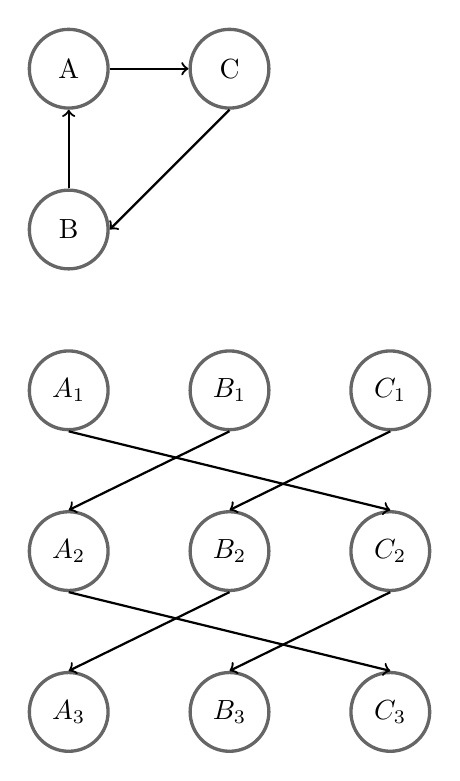
\begin{tikzpicture}[
roundnode/.style={circle, draw=black!60,  very thick, minimum size=10mm},
squarednode/.style={rectangle, draw=red!60, fill=red!5, very thick, minimum size=5mm},
]
%Nodes
\node[roundnode]      (A)                    {A};
\node[roundnode]      (B)       [below=of A] {B};
\node[roundnode]      (C)       [right=of A] {C};

 
%Lines
\draw[thick,->] (B.north) -- (A.south);
\draw[thick,->] (A.east)  -- (C.west);
\draw[thick,->] (C.south) -- (B.east);

%Nodes
\node[roundnode]      (A1)       [below=of B]  {$A_1$};
\node[roundnode]      (B1)       [right=of A1] {$B_1$};
\node[roundnode]      (C1)       [right=of B1] {$C_1$};

\node[roundnode]      (A2)       [below=of A1]             {$A_2$};
\node[roundnode]      (B2)       [right=of A2] {$B_2$};
\node[roundnode]      (C2)       [right=of B2] {$C_2$};

\node[roundnode]      (A3)       [below=of A2]             {$A_3$};
\node[roundnode]      (B3)       [right=of A3] {$B_3$};
\node[roundnode]      (C3)       [right=of B3] {$C_3$};
 
%Lines
\draw[thick,->] (A1.south) -- (C2.north);
\draw[thick,->] (B1.south) -- (A2.north);
\draw[thick,->] (C1.south) -- (B2.north);

\draw[thick,->] (A2.south) -- (C3.north);
\draw[thick,->] (B2.south) -- (A3.north);
\draw[thick,->] (C2.south) -- (B3.north);

\end{tikzpicture}
\end{center}
\caption{Conversion of a cyclic graph into a DAG. A similar process will convert the eight-connected grid into a DAG.}
\end{figure}
  
\begin{figure}[!h]
\label{speye}
\centering
\includegraphics[scale=0.8]{speye.png}
\caption{Placement of non-zero entries for a 2x2 and a 4x4 adjacency matrix. NZ is the number of non-zero entries in the adjacency matrix}
\label{fig_sim}
\end{figure}

Topological order of the nodes is critical for dynamic programming \cite{(Dynamic Programming book)}, and it needs to be in the reverse of the eventual path taken. 
So, the ordering of nodes begins with the target in the lower right, then moves radially out from this corner. 
This scheme will be affected by the connections between grid cells. 
Choosing an eight-connected grid allows for a relatively simple ordering scheme. 
The order needs to be such that as the algorithm progresses from target node to start node, the cost at each successive node depends only on nodes that have already been completely considered. 

\begin{figure}[h]
\begin{center}

\newcommand\setrow[5]{
\setcounter{col}{1}
\foreach \n in {#1, #2, #3, #4, #5} {

	\edef\x{\value{col} - 0.5}
	\edef\y{5.5 - \value{row}}
	\node[anchor=center] at (\x, \y) {\n};
	\stepcounter{col}
	}
	\stepcounter{row}
}


\begin{tikzpicture}%[scale=0.5]
\label{node-ordering}
\begin{scope}[font=\sffamily\slshape]
\draw (0,0) grid (5,5);

\setcounter{row}{1}
\setrow {25}{24}{22}{19}{15}
\setrow {23}{21}{18}{14}{10}
\setrow {20}{17}{13}{9}{6}
\setrow {16}{12}{8}{5}{3}
\setrow {11}{7}{4}{2}{1}
\end{scope}

\end{tikzpicture}

\end{center}
\caption{Ordering of nodes for an adjacency matrix with the starting node in the upper left and ending node in the lower right. The topological order of nodes should expand outward starting with the target node. }
\end{figure}  
The algorithm moves through the adjacency matrix one column at a time, in topological order. 
Each column represents a map region and a path step number. 
The unwrapping procedure means that the first $N$ columns represent each node at the first entry in any path, the next $N$ columns represent the nodes at step two in any path, etc. where $N$ is the number of map regions.
At each column, cost and probability of traverse for all connections going to that column are calculated. 
These values are concatenated with the existing list of paths at that node (if any) and the Pareto front of non-dominated paths is saved. 
The front consists of the paths with the lowest cost and highest $P_{tr}(x)$. 
Once the algorithm has completed, there is a saved list of paths on the Pareto front from each node to the target node.
After the algorithm completes, the output will need to be 're-wrapped.' 
This process will take each path in the adjacency matrix and associate it with a specific map region.
This is the opposite of the un-wrapping procedure shown in figure \ref{DAG}. 
Some heuristic or metric is then used to select a single best path from this front at each node.
The output of the algorithm is a list of paths from each node to the target node. 
Each path is a set of waypoints located at the center of map regions. 

\subsection{Environmental Metrics}
Each grid segment has several metrics associated with it. These metrics are averaged over an entire grid cell, so they are each a function of position in the map and area covered by a cell.

These are probability of traverse ($P_{tr}$), obstacle density ($\mu$), and harvested energy ($E_h$). Probability of traverse reflects the dispersion of obstacles throughout a segment. 
Dispersion is defined as in the Euclidean dispersion discussed in \cite{lavalle2004relationship}, which is the radius of the largest ball that fits into the segment without touching an obstacle. 
A larger value of dispersion indicates that the robot is more likely to successfully navigate through a grid segment.
This probability of traverse can be multiplied among sequential map segments to calculate the probability that the robot will get stuck while moving from one segment to another, as in equation \ref{Ptr}. 
A segment covered entirely by a known obstacle, for example a river if the vehicle is a wheeled robot, would have $P_{tr} = 0$. 

Obstacle density is defined as the ratio of area covered by obstacles in a map segment to the total area of that segment. 
This metric is used to calculate the cost function, and reflects the likelihood that the actual path will need to deviate from a straight line through the map segment. 

Harvested energy is a function of the available energy in a grid segment. Both the intensity and the type of energy are reflected in this measure; the availability of geothermal energy is not factored into the cost function for a robot which does not carry a transducer to harvest that energy.
 
\subsection{Cost Function}
The cost function is used to give an estimate of total energy usage between two points. 
Therefore, it is entirely dependent on the vehicle model used. Dong and Sun \cite{minimizing energy consumption of wheeled mobile robots ...} propose the following cost function based on power usage for movement of wheeled vehicles:
\begin{equation}
J_i = J_{i-1} + 2\mu_{i-1,i}mg s_{i-1,i}
\end{equation}
where $\mu$ denotes the frictional coefficent, $i$ is the node index, $m$ is mass, $g$ is the gravitational acceleration, and $s$ is the distance between points. 
Additionally, they use a penalty function which affects the cost function as the path moves near an obstacle.
Mei et al. \cite{Mei - deployment} note that in addition to motion there are energy costs associated with sensing and computing power, which are relatively constant over time (provided that the usage rate is constant).
They also build the energy model for each vehicle empirically.

To account for the possibility that the ground path of the robot (the actual path taken) may not be a straight line from the center of one map region to the next, we introduce an obstacle density $\mu(x_i)$. 
A higher density of obstacles within a region increases the likelihood that the robot will need to deviate from a straight line path. 
In building the cost function we assume that the length ground path increases proportionally to the obstacle density.

For a generic wheeled vehicle, the cost function used to evaluate each cell in EAPP is:

\begin{equation}
H_i = (1 + \mu(x_i))(\delta_i s_{i} + E_c + E_s - E_{h_i})
\end{equation}
where $l_i$ is the width of the cell, $\mu(x)_i$ is the obstacle density in a grid cell, $\delta_i$ is the estimated incremental cost of driving on the the surface of the cell, $E_c$ and $E_s$ are the estimated computing and sensing costs respectively, and $E_h$ is the estimated energy harvested by the robot from the environment. 
The cost $\delta_i$ is built up empirically, by driving the vehicle on multiple surfaces with different coefficients of friction and inclines.
Estimated $\delta_i$ in a grid cell comes from the satellite image, which is used to determine type of surface. 
The robot should have an internal model of types of surfaces to use, and by comparing the surface type with this  look-up table will give the incremental cost.
Some modification may be appropriate for different vehicle types, if specific motions require a higher energy. 
For example, treaded vehicles require more power for turning than for going straight, due to the additional sliding friction.
The total cost of a path is the summation of the cost of each included cell: 
\begin{equation}
J(x) = \sum_{i=1}^k H_i
\end{equation}
where in this case $k$ is the number of cells traversed by a given path $x$.

\subsection{Assumptions}
\subsubsection{Availability of local navigation algorithm:} The algorithm presented in this paper assumes the availability of a local algorithm, as discussed in the algorithm description. 
The local algorithm must act while the robot is moving to follow waypoints provided by the global algorithm, and it must avoid obstacles. 
However, in the case that the robot's actual path deviates from the waypoints due to obstacles, a new path is easily generated from the current node to the target. 
In fact, the algorithm returns the Pareto front of non-dominated paths from each node to the target node, and these are easily stored in a lookup table. 

\subsubsection{No negative weight cycles are present in graph:}
There must not be any negative weight cycles present in the original graph, although zero-weight cycles are allowed. A cycle is defined as any path segment containing more than one node which begins and ends in the same location.  So for all path segments describing a cycle, 
\begin{equation}
\sum_{i=1}^n J_i(x) > 0,\ n>1
\end{equation}
for any path segment that starts and ends at the same node.

We assert that this is a realistic assumption for any map. Any on-board battery has a set capacity, and once SOC reaches 100\% no additional energy can be harvested until some is expended. 
As harvested energy ($E_h$) is the only negative term in the cost function, this means that there can be no infinite negative weight cycles. 
The assumption of no negative weight cycles is then reasonable. 
The case of a zero weight cycle can be handled by adding a small penalty each time a path returns to a grid segment that it has already visited.
In our test environment, there are no zero-weight cycles and therefore no penalty due to the relatively low value of harvested energy compared to the cost of movement.

\subsubsection{Availability of map data:}
Map data must be available as input to the algorithm. 
This means both a satellite image and the image processing capability to estimate environmental parameters. 
While the design of the algorithm attempts to limit the required information to that which is typically available, there is no guarantee that this information is always available or that the image processing is always accurate. The lack of representative data will affect the performance of the algorithm.

\subsection{Pseudocode}
The pseudocode for the algorithm is given in this section. The subfunctions used in the algorithm are described below. 
Note that the loop beginning in line 3 must run in reverse, beginning with the column containing the goal node.

Inputs to the algorithm are: $\mathcal{G}$, the graph of connections between grid cells; $v_{target}$, the index of the target cell; and $\epsilon_c$, the minimum acceptable value of $P_{tr}$ for a path. The variable definitions are: $v$, $b$, and $path$ refer to a single path; $D$ is a list storing the Pareto front of best paths leading to each 'unwrapped' node in the adjacency matrix (including the path $v$ and the values for cost and $P_{tr}$ associated with it), $F$ stores the Pareto front of best paths for each 'rewrapped' node, and the pareto front for a single node is referred to as $D_{col}$.
\bigskip

\textsc{EAPP}($\mathcal{G}, v_{target}, \epsilon_c$)
\begin{algorithmic}[1]
\STATE $D:=\{\}$ \COMMENT{the pareto front of paths leading to each node}
\STATE \textbf{adj} $\leftarrow$ \textbf{BUILD\_ADJACENCY}($\mathcal{G}$)
\FORALL {$col$ in adj}
\STATE $C =$ \textbf{FIND\_CONNECTIONS($col$)}
\FORALL {$v$ in $C$}
\STATE $v  \leftarrow v \cup col$ 
\STATE $new\_c \leftarrow$ \textbf{COST}($v$)
\IF {$new\_c.P_{tr} > \epsilon_c$} 
\STATE $new\_c.cost += penalty $ 
\ENDIF
\STATE $C \leftarrow C \cup new\_c$ 
\STATE $D_{col} = $\textbf{PARETO($C)$}
\ENDFOR
\ENDFOR
\STATE $F \leftarrow \textbf{RE\_WRAP}(D)$
\STATE $paths \leftarrow \textbf{EXTRACT\_PATHS\_TO\_GOAL}(F, v_{target})$
\FORALL {paths}
\IF {$path.SOC \leq 0$}
\STATE $path = \emptyset$
\ENDIF
\ENDFOR
\STATE $b \leftarrow \textbf{CHOOSE\_BEST\_PATHS}(paths)$
\RETURN $b$
\end{algorithmic}

\subsubsection{BUILD\_ADJACENCY($\mathcal{G}$)} creates the adjacency matrix $A$ from the connected graph by the unwrapping procedure described in a previous section.
\subsubsection{FIND\_CONNECTIONS($col$)} returns the list of nodes that connect to $col$. This means any non-zero entry in the column of the adjacency matrix corresponding to the current node, $col$.
\subsubsection{COST($v$)} calculates and returns the total cost, $P_{tr}(x)$, and estimated remaining SOC for the node $v$. The cost here relates the ending node of a given path and the current node $v$. As it is built in reverse, the estimate of SOC is only valid once the path reaches the first node of the adjacency matrix (meaning it contains one possible starting node).
\subsubsection{PARETO($C$)} builds the pareto front of non-dominated paths from all of the paths passed to it. If the nodes are in the front they are returned, otherwise they are removed.
\subsubsection{RE\_WRAP($D$)} reverses the 'unwrapping' procedure which happens when the adjacency matrix is created. 
The function finds and returns the Pareto front of best paths for each map region, regardless of the number of steps in each path. 
\subsubsection{EXTRACT\_PATHS\_TO\_GOAL($D, v_{target}$)} returns all viable paths from the list $D$ for the given node $v_{target}$
These consist of any path which begins with a node in the first row of the adjacency matrix and also contains $v_{target}$. 
To speed execution, an additional check can be added in the main algorithm which removes a node from the list $C$ once it contains the target node. 
If this check is not present, then any nodes in a path which come after $v_{target}$ are ignored in this function.
\subsubsection{CHOOSE\_BEST\_PATH($paths$)} returns the single best path from the pareto front for each node. 'Best' is a user-defined metric, and may be some combination of cost and probability of traverse. For this paper it is simply the lowest-cost path in each Pareto front.

\subsection{Dynamic programming:}
The primary contribution of this work is in the problem definition; the use of $P_{tr}(x)$ and $\mu(x)$ to separate energy costs from probability of traverse is novel, and it is possible to design many types of navigation algorithm which use these measures. 
The proposed dynamic programming algorithm presents several advantages over competing approaches.
The primary advantage is that the proposed algorithm considers every possible path of length $n$ or less, meaning that the results are globally optimal according to the cost function and within the constraint. 
Additionally, the results of the algorithm are a choice of paths from each node to the target node, greatly reducing the burden on the local navigation algorithm.
The segmented grid approach is flexible, and estimates of environmental parameters can be improved by refining individual sections of the grid. There is no need for square or homogenously sized grid sections, it is merely a convenience.
The algorithm is deterministic, so the same results are returned regardless of whether the algorithm is run on-board a robot or remotely with the resulting waypoints transmitted to the robot.
Conversely, the proposed algorithm must be re-run if the threshold on $P_{tr}$ or the environmental costs change. 
The algorithm is also not anytime \cite{definition of anytime}, and its running time may preclude it from use with fast-moving vehicles such as Unmanned Arial Vehicles.

%\section{Theoretical Results}


\section{Simulation Results}
In this section we test the algorithm on a sample environment and discuss the results. The environment used is a section of Rock Creek Park in Washington, D.C. at coordinates: \textbf{coords}
A satellite image is pulled from (cite google maps?), and the map is broken up into equal area regions.
Each region is assigned a cost and a probability of traverse.

\begin{figure}[h!]
\label{cost_map}
\centering
\includegraphics[scale=1.5]{cost_map}
\caption{Cost function evaluated for each map region. A darker value indicates a higher cost.}
\end{figure}

\begin{figure}[h!]
\label{Ptr_map}
\centering
\includegraphics[scale=1]{P_tr_map}
\caption{Values of $P_{tr}$ associated with each map region. A darker value indicates a lower probability of traverse.}

\end{figure}


The algorithm is programmed into a MATLAB script file. 
The robot begins in the bottom left corner of the map and the target node is the top right corner.
The resulting best path is shown in figure [fig no].

\begin{figure}[h!]
\label{best_path}
\centering
\includegraphics[scale=1]{RCP_soln}
\caption{The best path through the environment. All possible connections are shown in blue, nodes are shown as stars, and the path chosen by EAPP is shown in red.}

\end{figure}

\section{Experimental Results}
In this section we present results using a mobile robotic platform in a simple environment. 
The environment consists of three different surfaces, each of which has an experimentally deternmined incremental cost.

\subsection{Robot Parameters}
\textbf{Conor's section}

\subsection{Implementation}
\textbf{Conor's section}

\subsection{Experimental Environment}
The test environment is represented in figure [fig no] by the cost and probability of traverse for each map region. 
The three different surfaces have different coefficients of friction, and are made of variously squishy? material which changes the cost associated with each region. 
In order to simulate a probability of traverse, obstacles placed in the environment were shifted slightly between runs. 
The probability of traverse is an estimate, as it would be for an environment only observed through satellite images.

\subsection{Results}
Using an identical map, we tested various starting and target positions. 
For each set of start and goal positions we tested a straight line path, a path which operates only in the lowest-cost region, and EAPP.
The paths are shown here, along with the normalized energy usage for each path. 


%\begin{figure}[!t]
%\centering
%\includegraphics[width=2.5in]{myfigure}
% where an .eps filename suffix will be assumed under latex, 
% and a .pdf suffix will be assumed for pdflatex; or what has been declared
% via \DeclareGraphicsExtensions.
%\caption{Simulation results for the network.}
%\label{fig_sim}
%\end{figure}

% An example of a double column floating figure using two subfigures.
% (The subfig.sty package must be loaded for this to work.)
%\begin{figure*}[!t]
%\centering
%\subfloat[Case I]{\includegraphics[width=2.5in]{box}%
%\label{fig_first_case}}
%\hfil
%\subfloat[Case II]{\includegraphics[width=2.5in]{box}%
%\label{fig_second_case}}
%\caption{Simulation results for the network.}
%\label{fig_sim}
%\end{figure*}
%
% Note that often IEEE papers with subfigures do not employ subfigure
% captions (using the optional argument to \subfloat[]), but instead will
% reference/describe all of them (a), (b), etc., within the main caption.
% Be aware that for subfig.sty to generate the (a), (b), etc., subfigure
% labels, the optional argument to \subfloat must be present. If a
% subcaption is not desired, just leave its contents blank,
% e.g., \subfloat[].


% An example of a floating table.
%\begin{table}[!t]
%% increase table row spacing, adjust to taste
%\renewcommand{\arraystretch}{1.3}
% if using array.sty, it might be a good idea to tweak the value of
% \extrarowheight as needed to properly center the text within the cells
%\caption{An Example of a Table}
%\label{table_example}
%\centering
%% Some packages, such as MDW tools, offer better commands for making tables
%% than the plain LaTeX2e tabular which is used here.
%\begin{tabular}{|c||c|}
%\hline
%One & Two\\
%\hline
%Three & Four\\
%\hline
%\end{tabular}
%\end{table}


\section{Conclusion}
This paper presents a global navigation algorithm that can extend the duration of deployment for wheeled mobile robots.
Our approach targets applications which require long-term autonomy and repetitive tasks, and it uses only information which may realistically be available in those scenarios.
We consider energy constraints on the robot, and account for harvesting energy from the environment in order to increase battery life. 
By introducing a recharging behavior where the robot seeks out a high-energy region and sits until its battery is full, it may be possible to extend the duration of deployment indefinitely.
Our method is tested in simulated and experimental environments, with results showing a significant improvement over more naive path choices.
EAPP separates probability of traverse from the energy-based cost function, allowing the algorithm to throw out paths which may be efficient but risk the loss of the robot.  





% if have a single appendix:
%\appendix[Proof of the Zonklar Equations]
% or
%\appendix  % for no appendix heading
% do not use \section anymore after \appendix, only \section*
% is possibly needed

% use appendices with more than one appendix
% then use \section to start each appendix
% you must declare a \section before using any
% \subsection or using \label (\appendices by itself
% starts a section numbered zero.)
%


%\appendices
%\section{Proof of the First Zonklar Equation}
%Appendix one text goes here.

% you can choose not to have a title for an appendix
% if you want by leaving the argument blank
%\section{}
%Appendix two text goes here.


% use section* for acknowledgment
\section*{Acknowledgment}


The authors would like to thank...


% Can use something like this to put references on a page
% by themselves when using endfloat and the captionsoff option.
\ifCLASSOPTIONcaptionsoff
  \newpage
\fi



% trigger a \newpage just before the given reference
% number - used to balance the columns on the last page
% adjust value as needed - may need to be readjusted if
% the document is modified later
%\IEEEtriggeratref{8}
% The "triggered" command can be changed if desired:
%\IEEEtriggercmd{\enlargethispage{-5in}}

% references section

% can use a bibliography generated by BibTeX as a .bbl file
% BibTeX documentation can be easily obtained at:
% http://mirror.ctan.org/biblio/bibtex/contrib/doc/
% The IEEEtran BibTeX style support page is at:
% http://www.michaelshell.org/tex/ieeetran/bibtex/
%\bibliographystyle{IEEEtran}
% argument is your BibTeX string definitions and bibliography database(s)
%\bibliography{IEEEabrv,../bib/paper}
%
% <OR> manually copy in the resultant .bbl file
% set second argument of \begin to the number of references
% (used to reserve space for the reference number labels box)

\bibliographystyle{IEEEtran}
\bibliography{mybib}
%\begin{thebibliography}{1}
%
%\bibitem{IEEEhowto:kopka}
%H.~Kopka and P.~W. Daly, \emph{A Guide to \LaTeX}, 3rd~ed.\hskip 1em plus
%  0.5em minus 0.4em\relax Harlow, England: Addison-Wesley, 1999.
%
%\end{thebibliography}

% biography section
% 
% If you have an EPS/PDF photo (graphicx package needed) extra braces are
% needed around the contents of the optional argument to biography to prevent
% the LaTeX parser from getting confused when it sees the complicated
% \includegraphics command within an optional argument. (You could create
% your own custom macro containing the \includegraphics command to make things
% simpler here.)
%\begin{IEEEbiography}[{\includegraphics[width=1in,height=1.25in,clip,keepaspectratio]{mshell}}]{Michael Shell}
% or if you just want to reserve a space for a photo:

%\begin{IEEEbiography}{Michael Shell}
%Biography text here.
%\end{IEEEbiography}

% if you will not have a photo at all:
%\begin{IEEEbiographynophoto}{John Doe}
%Biography text here.
%\end{IEEEbiographynophoto}

% insert where needed to balance the two columns on the last page with
% biographies
%\newpage

%\begin{IEEEbiographynophoto}{Jane Doe}
%Biography text here.
%\end{IEEEbiographynophoto}

% You can push biographies down or up by placing
% a \vfill before or after them. The appropriate
% use of \vfill depends on what kind of text is
% on the last page and whether or not the columns
% are being equalized.

%\vfill

% Can be used to pull up biographies so that the bottom of the last one
% is flush with the other column.
%\enlargethispage{-5in}



% that's all folks
\end{document}


